\documentclass[12pt]{beamer}
\usepackage[utf8]{inputenc}
\usepackage[spanish]{babel}
%\usepackage[dvips]{epsfig}
\usepackage{graphics}
\usepackage{url}
\usepackage{ulem}
\usepackage{beamerthemesplit}
\usepackage{color}
\usepackage{hyperref}
\usepackage{wrapfig}
\usetheme{CambridgeUS}
\setbeamercovered{transparent}

\title{User identification with username and password in structured P2P networks}
\subtitle{}
\author[R. Fernández]{Rodrigo Fernández \\ \small{\texttt{rfernand@inf.utfsm.cl}}}
\institute[]{Universidad Técnica Federico Santa María}
\titlegraphic{
\includegraphics[height=1cm]{img/logo}}
\date{\today}

\begin{document}
\bibliographystyle{plain}
  \frame{\titlepage}
  \frame{\tableofcontents}
	\section{}
  \section{General formulation of the problem and thesis proposal}
  \subsection{Context and Motivation}

  \begin{frame}
  \frametitle{P2P Networks}
  \framesubtitle{Characteristics}
  \begin{table}
  \begin{tabular}{p{7cm}p{3cm}}
  \begin{itemize}
    \item Scalable
    \item Decentralized
    \item Self-maintained
    \item Robust
  \end{itemize}
  &
  \vspace{1.5cm}
  \includegraphics[width=4cm]{../../presentacion/img/p2p-unstructured}\\
  \end{tabular}
  \end{table}
  \end{frame}
  
  \begin{frame}
  \frametitle{P2P Networks}
  \framesubtitle{Overlay structure}
  \begin{table}
  \begin{tabular}{p{7cm}p{3cm}}
  \begin{itemize}
      \item Structured networks (CAN, CHORD)
      \item Unstructured networks (Gnutella, Bittorrent)
  \end{itemize}
  &
  \vspace{1.5cm}
  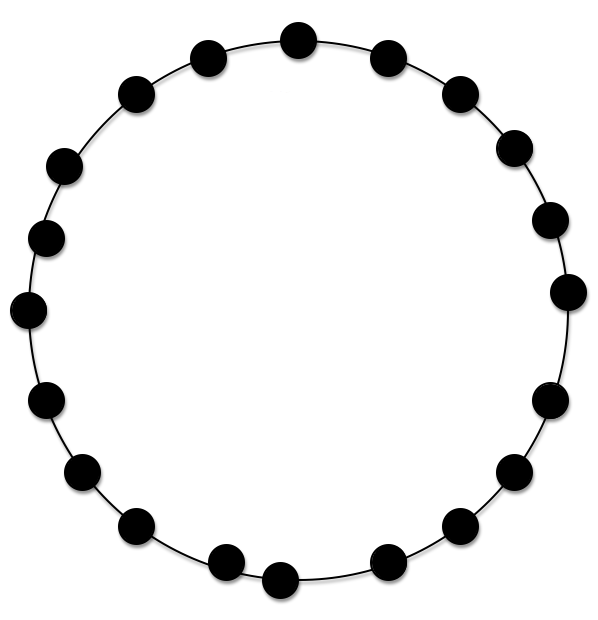
\includegraphics[width=4cm]{../../presentacion/img/p2p-structured}\\
  \end{tabular}
  \end{table}
  \end{frame}
  
  \begin{frame}
  \frametitle{P2P Networks}
  \framesubtitle{Overlay structure}
  \begin{table}
  \begin{tabular}{p{7cm}p{3cm}}
  \begin{itemize}
      \item Images of structured/unstructures networks
      \item Differences
  \end{itemize}
  &
  \vspace{1.5cm}
  
\includegraphics[width=4cm]{../../presentacion/img/example}\\
  \end{tabular}
  \end{table}
  \end{frame}
  
  \begin{frame}
  \frametitle{Username / password identification}
  \framesubtitle{Why?}
  \begin{table}
  \begin{tabular}{p{7cm}p{3cm}}
  \begin{itemize}
    \item Many \textbf{complex systems} require authenticated users to work.
    \item Most of the users has \textbf{more than one device}, so identification through
      multiple devices is needed.
    \item \textbf{User are accostumed} to username/password solutions.
  \end{itemize}
  &
  \vspace{1.5cm}
  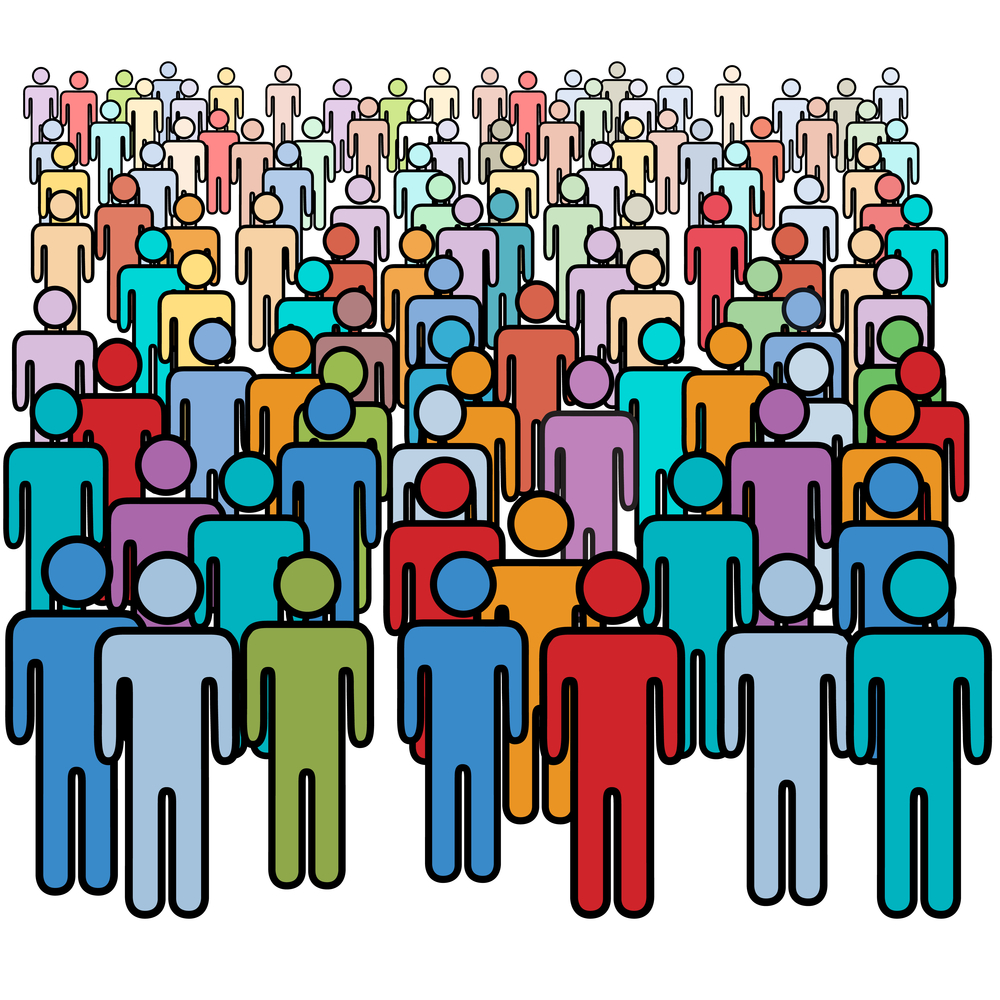
\includegraphics[width=4cm]{../../presentacion/img/users}\\
  \end{tabular}
  \end{table}
  \end{frame}
  
  \begin{frame}
  \frametitle{Username / password identification}
  \framesubtitle{P2P Identification Schemes}
  
    Descentralized schemes distributes the task of public key auth to all
    participants.
  \begin{table}
  \begin{tabular}{p{7cm}p{3cm}}
  \begin{itemize}
    \item PGP-like scheme\\ Creates web of trust to auth public keys based on
      their acquaintances opinions.
    \item Quorum-based scheme\\ Multiple independent participants replicate
      public keys.
  \end{itemize}
  &
  \vspace{1.5cm}
  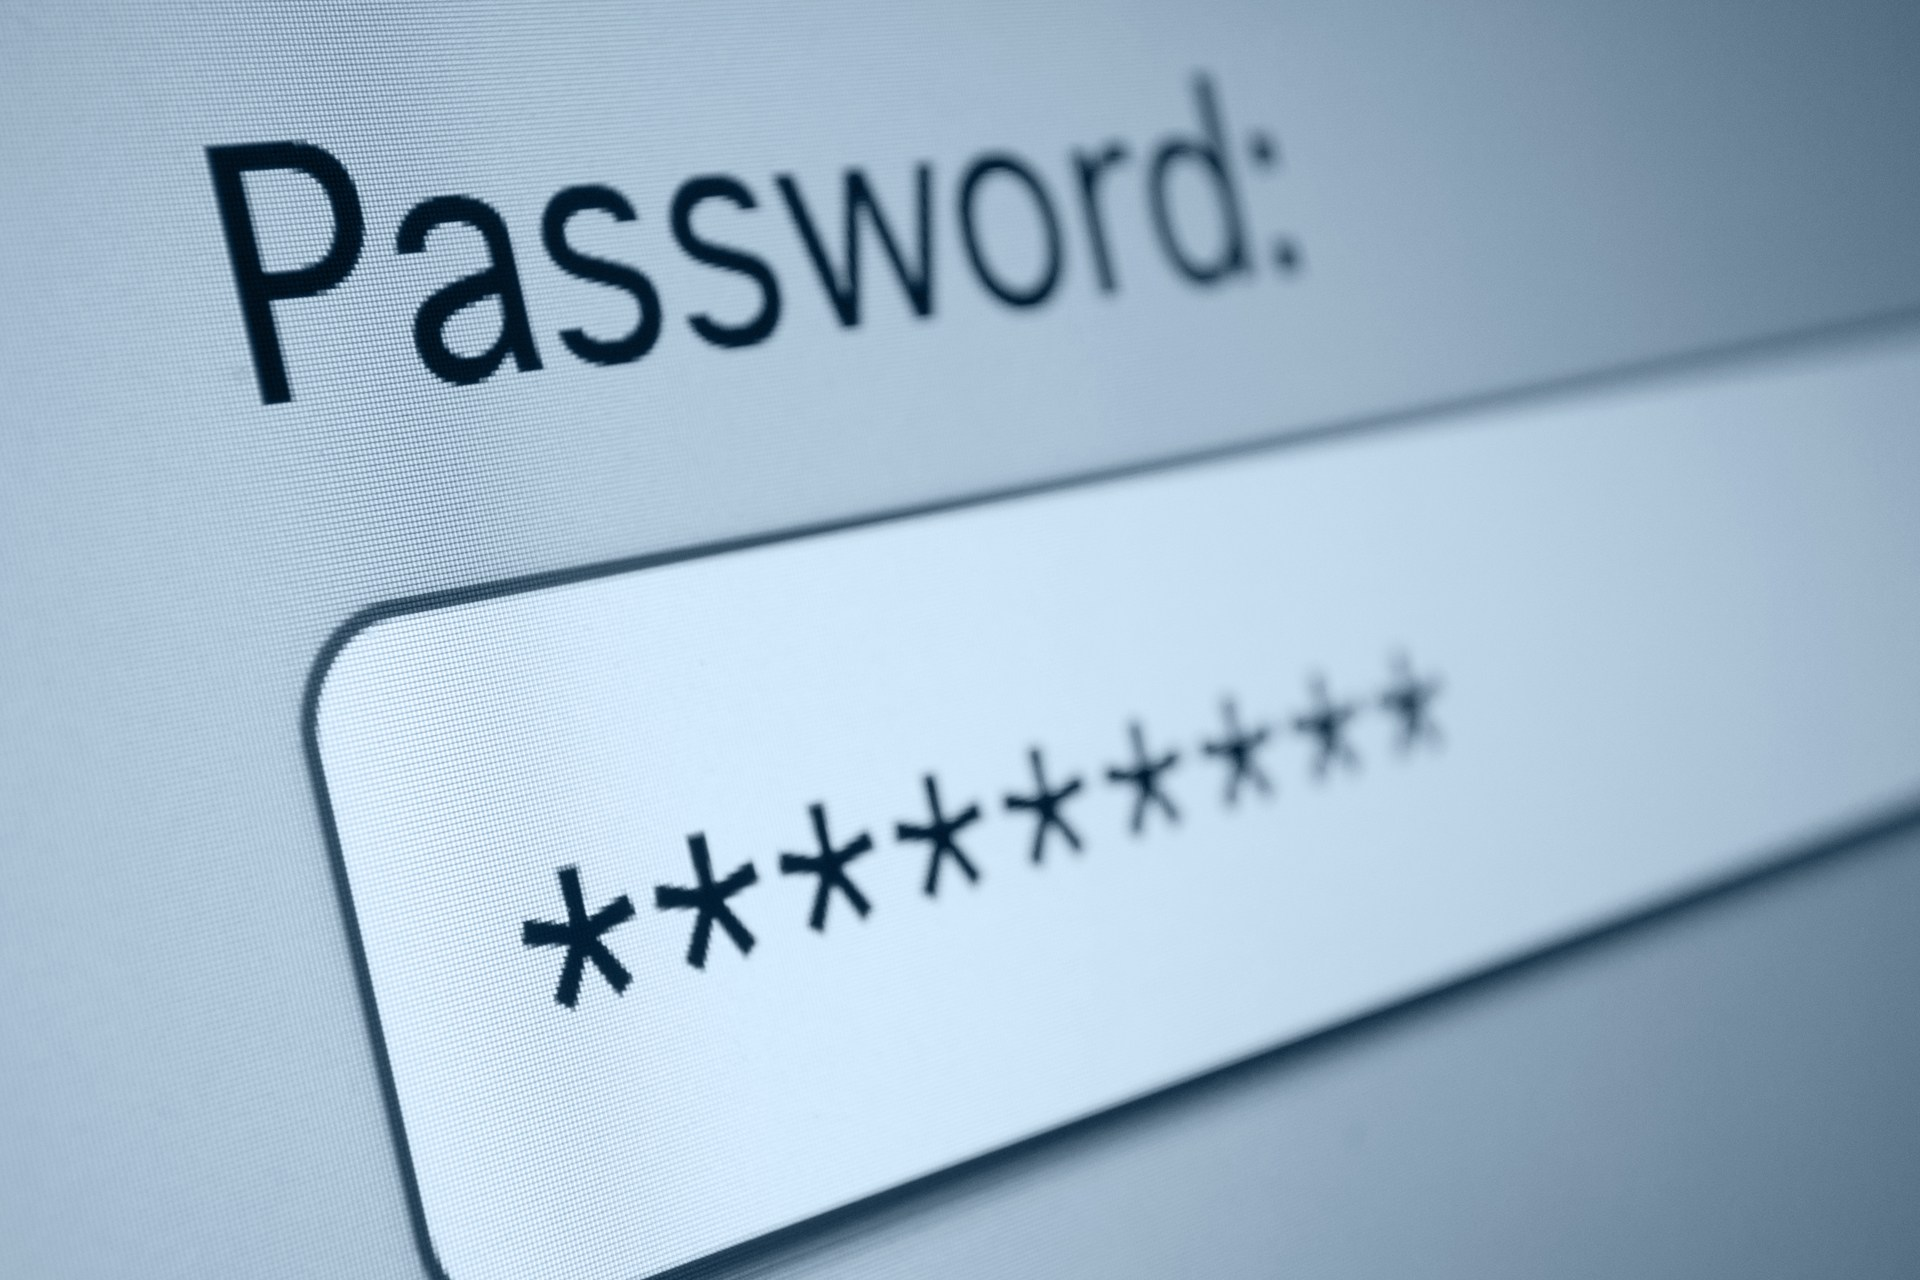
\includegraphics[width=4cm]{../../presentacion/img/password}\\
  \end{tabular}
  \end{table}
  \end{frame}
  
  \begin{frame}
  \frametitle{Identification schemes}
  \framesubtitle{In need of a third party}
  \begin{table}
  \begin{tabular}{p{7cm}p{3cm}}
  \begin{itemize}
      \item PKI
      \item Username/password pair
  \end{itemize}
  
  Poor scaling, single point of failure, heavy administration overhead.
  &
  \vspace{1.5cm}
  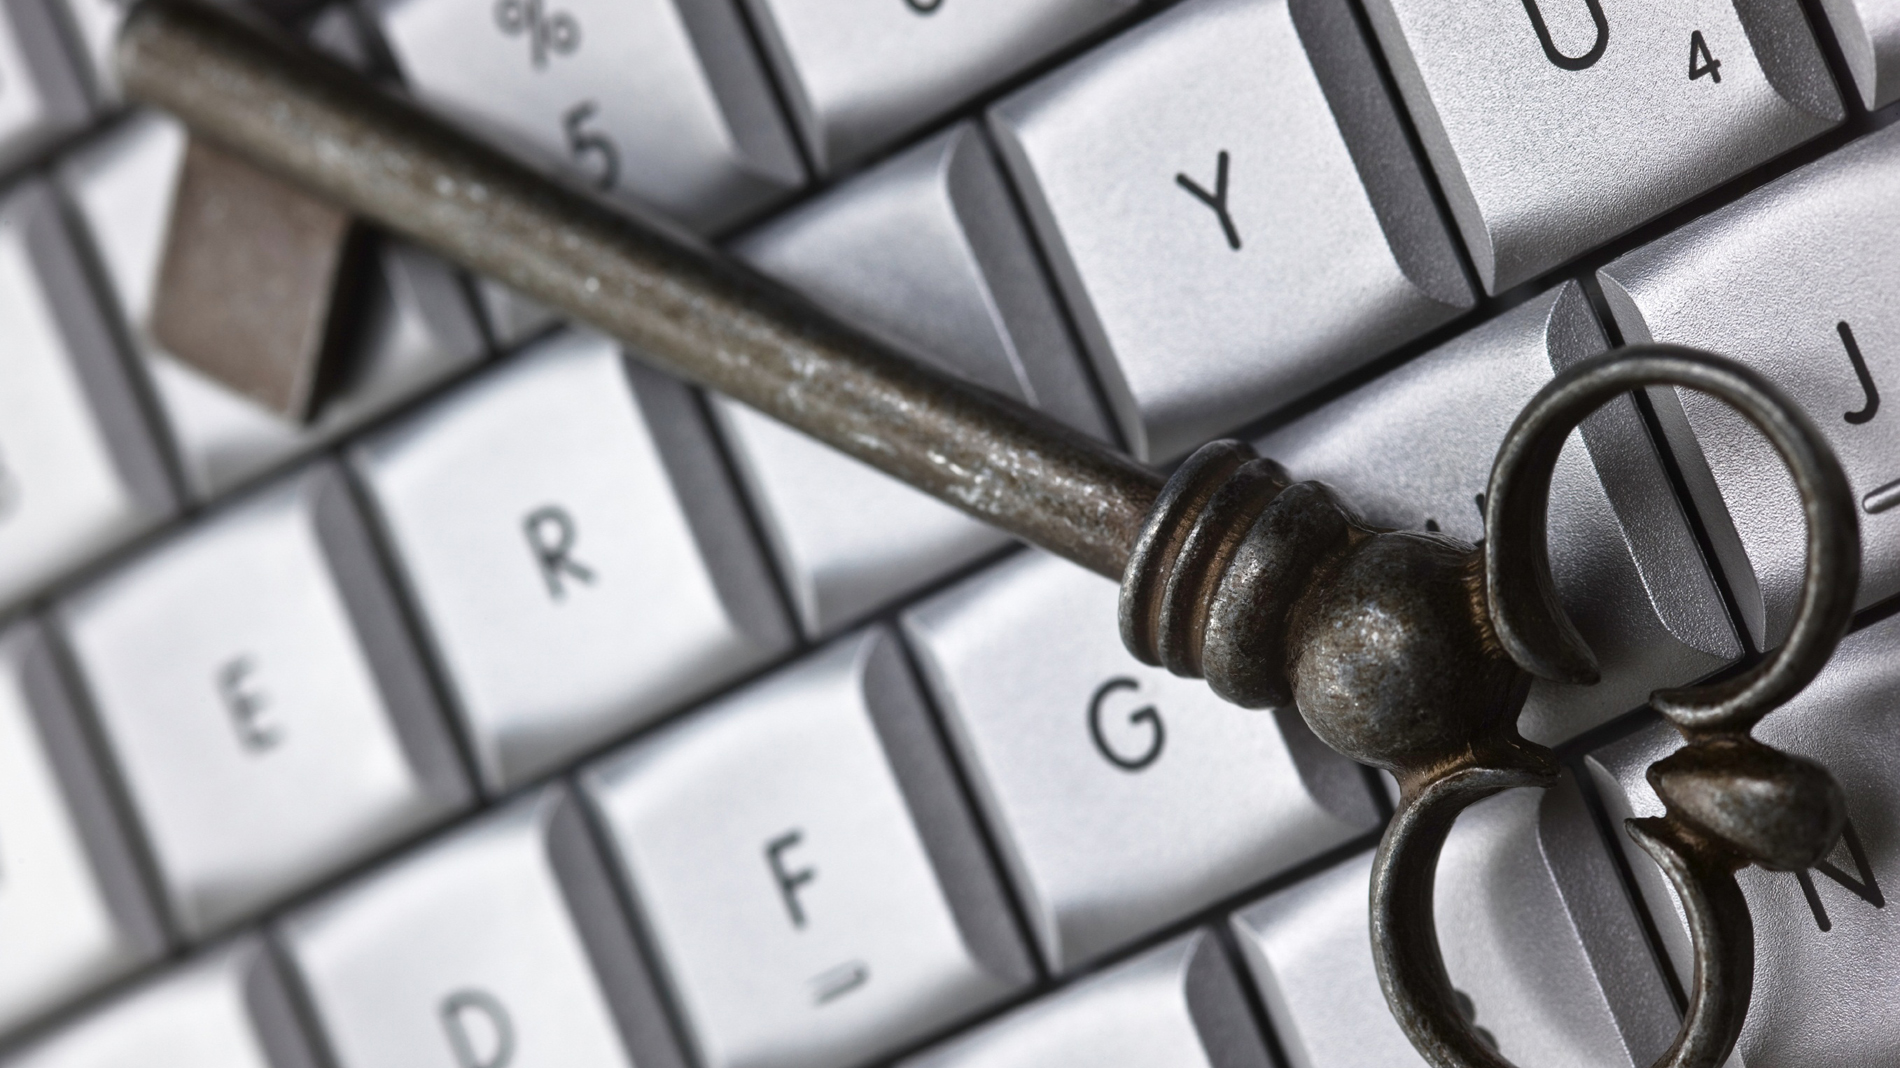
\includegraphics[width=4cm]{../../presentacion/img/keyboard_key}\\
  \end{tabular}
  \end{table}
  \end{frame}
  
  \begin{frame}
  \frametitle{Trust in P2P networks}
  \begin{table}
  \begin{tabular}{p{7cm}p{3cm}}
  \begin{enumerate}
      \item To deliver a valuable service in P2P applications, it
  is important to trust that the participants will act as requested.
      \item We need to be sure that other peers will forward
  messages, and that the designated peers will indeed save the information
  correctly so that operations can be successful.
  \end{enumerate}
  &
  \vspace{1.5cm}
  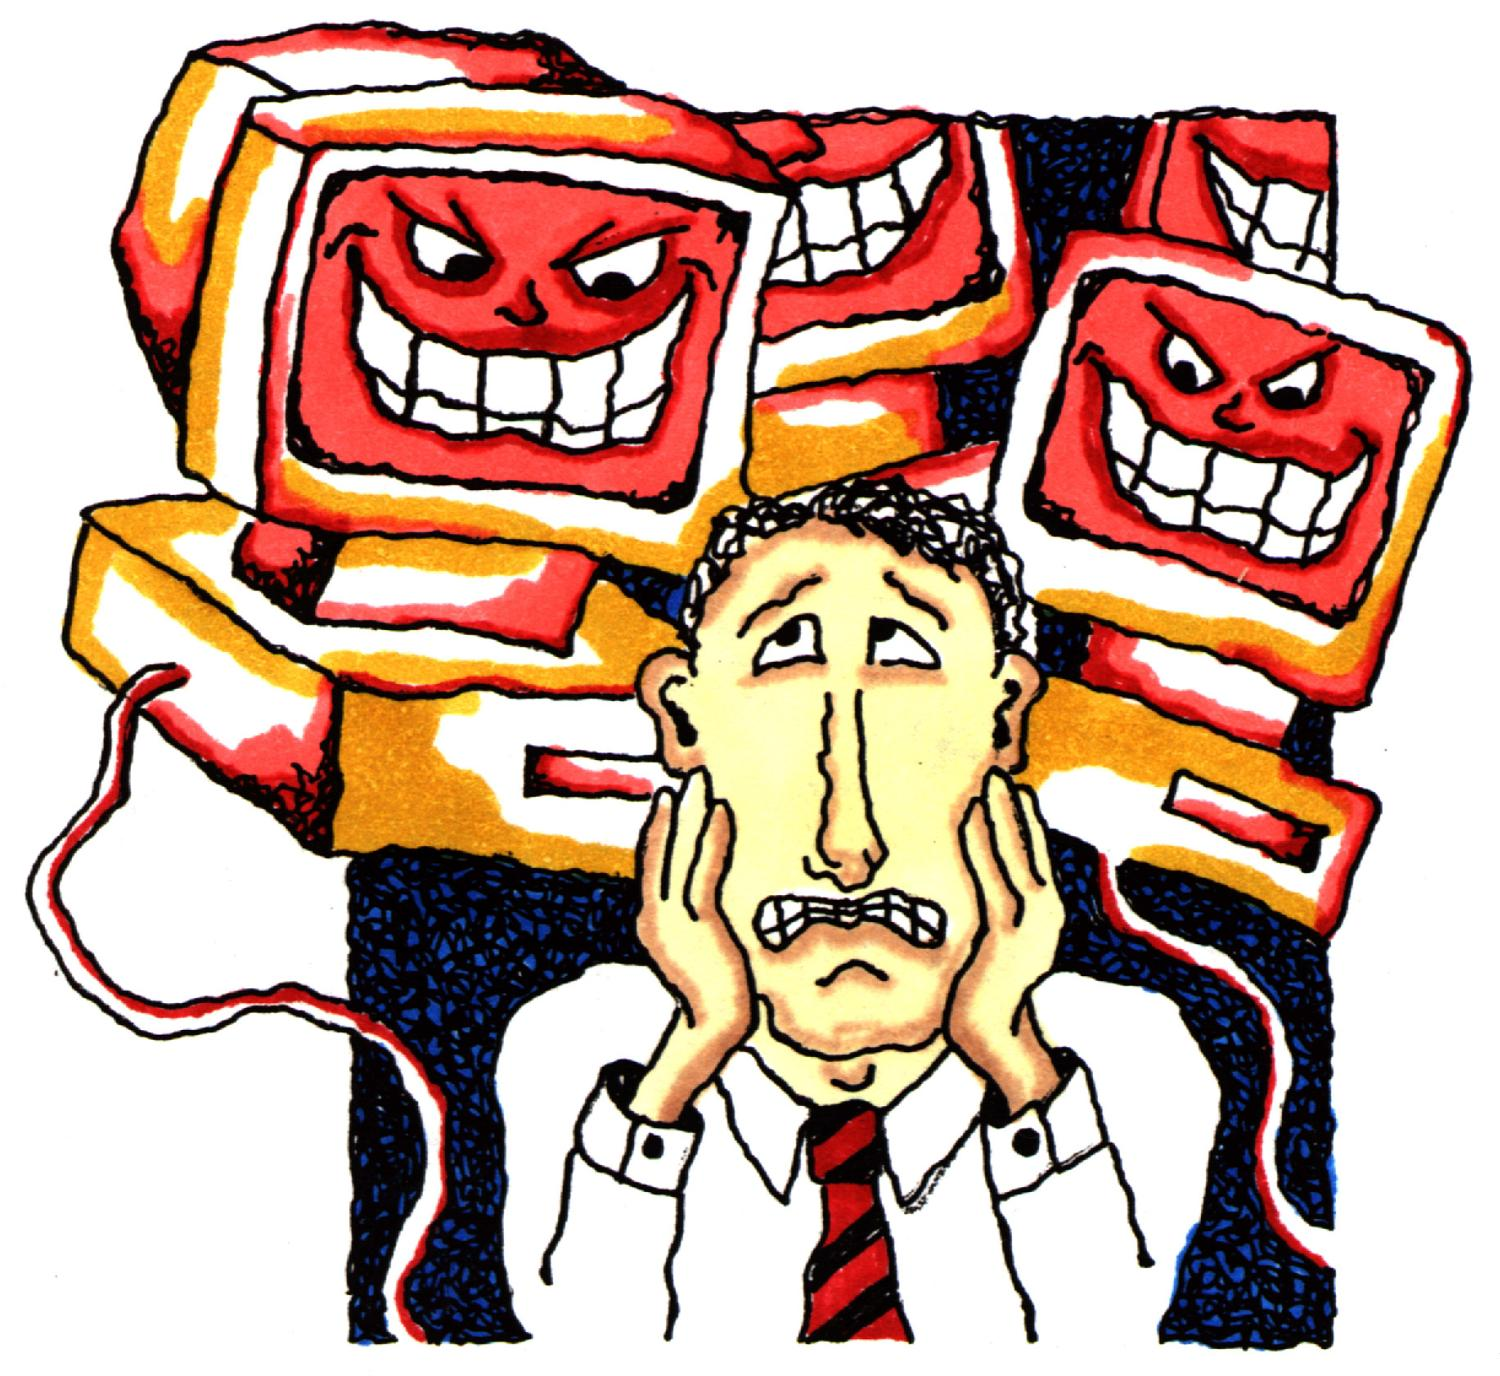
\includegraphics[width=4cm]{../../presentacion/img/malicious}\\
  \end{tabular}
  \end{table}
  \end{frame}
  
  \begin{frame}
  \frametitle{Trust in P2P networks}
  \framesubtitle{Building Trust}
  %Consequently, the quality of service of applications may
  %be deteriorated due to message overhead or data loss.
  \begin{table}
  \begin{tabular}{p{7cm}p{3cm}}
  \begin{enumerate}
      \item Complex since a P2P network includes untrusted nodes from an open environment.
      \item Untrusted nodes may be faulty, malicious, and act together to attack the network.
  \end{enumerate}
  &
  \vspace{1.5cm}
  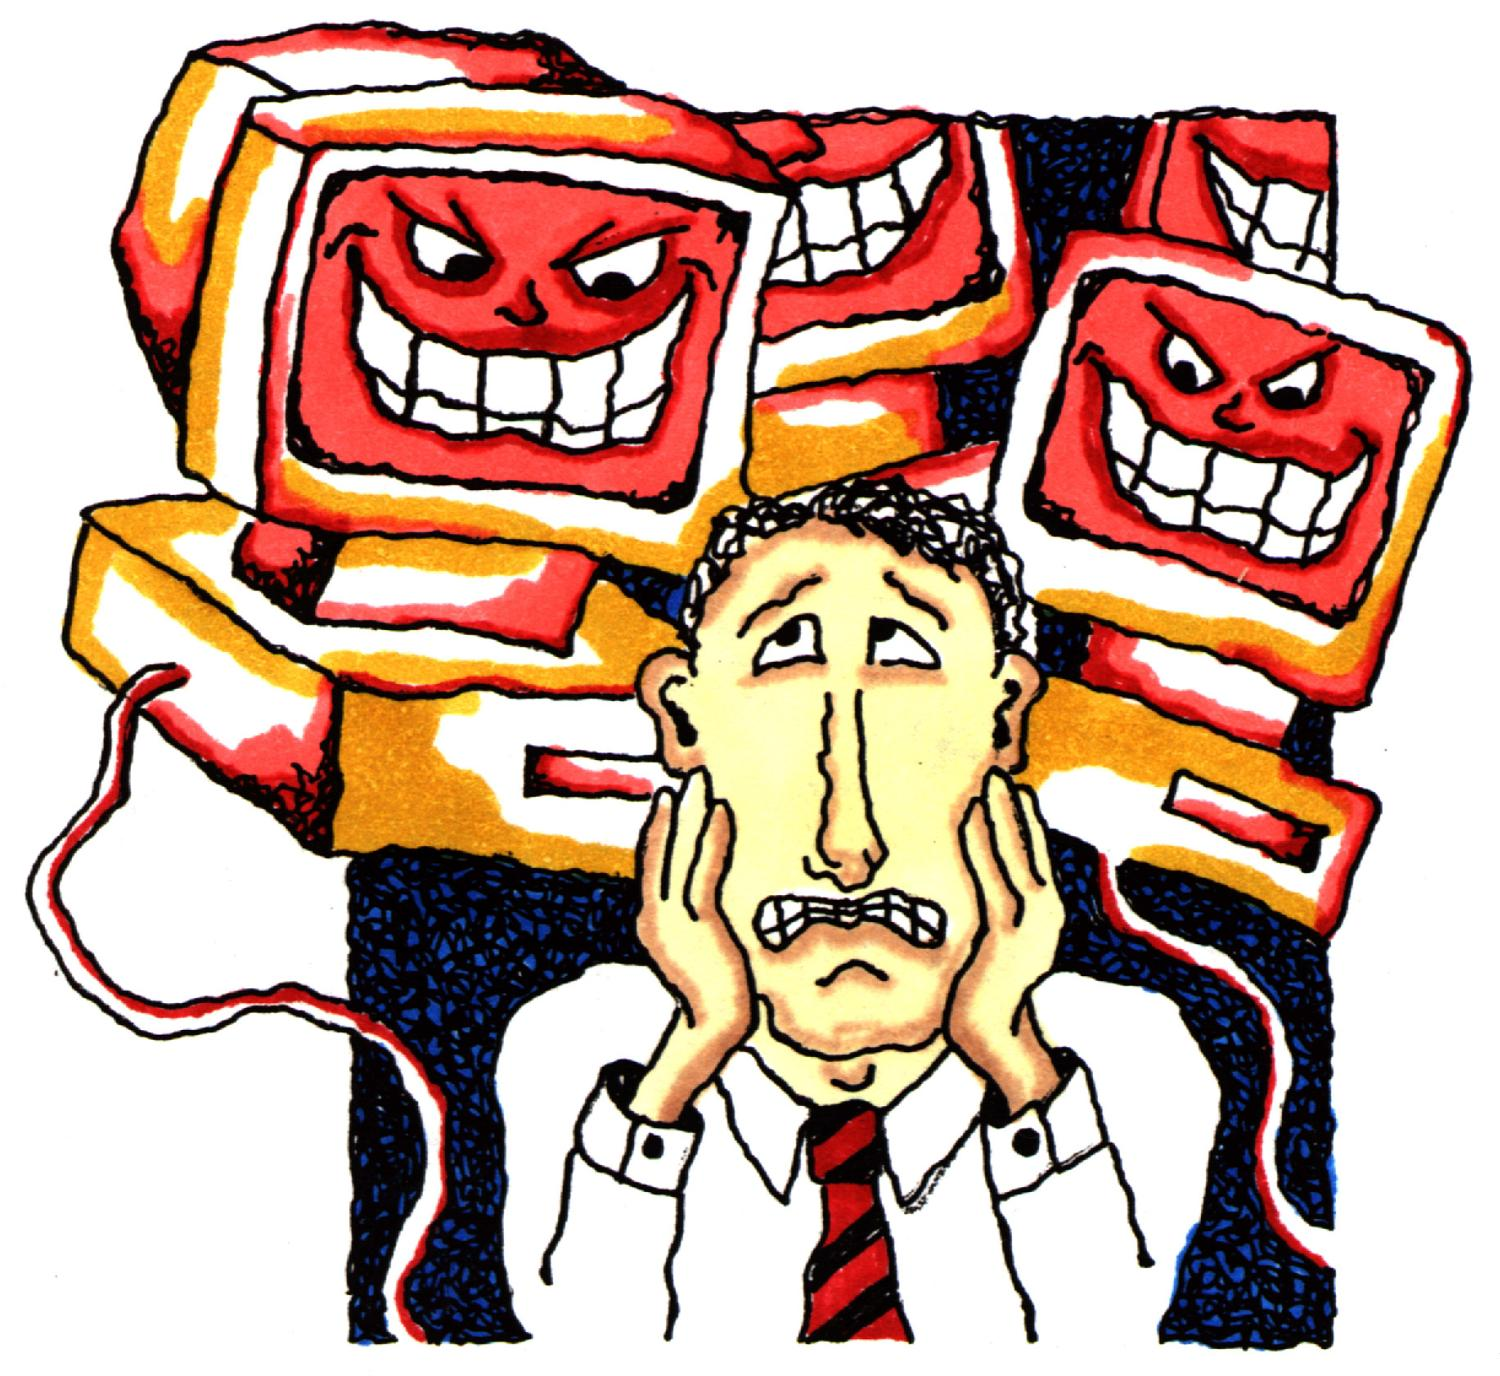
\includegraphics[width=4cm]{../../presentacion/img/malicious}\\
  \end{tabular}
  \end{table}
  \end{frame}
  
  \begin{frame}
  \frametitle{Trust in P2P networks}
  \framesubtitle{How to detect faulty nodes?}
  %Consequently, the quality of service of applications may
  %be deteriorated due to message overhead or data loss.
  \begin{table}
  \begin{tabular}{p{7cm}p{3cm}}
  \begin{description}
      \item{Reputation systems:} Assess the past history of a
  peer by gathering feedback from nodes with previous interactions with this
  peer.
      \item{Accountability:} Detects and exposes faulty nodes by
  creating non-repudiable records of every node’s actions.
  \end{description}
  &
  \vspace{1.5cm}
  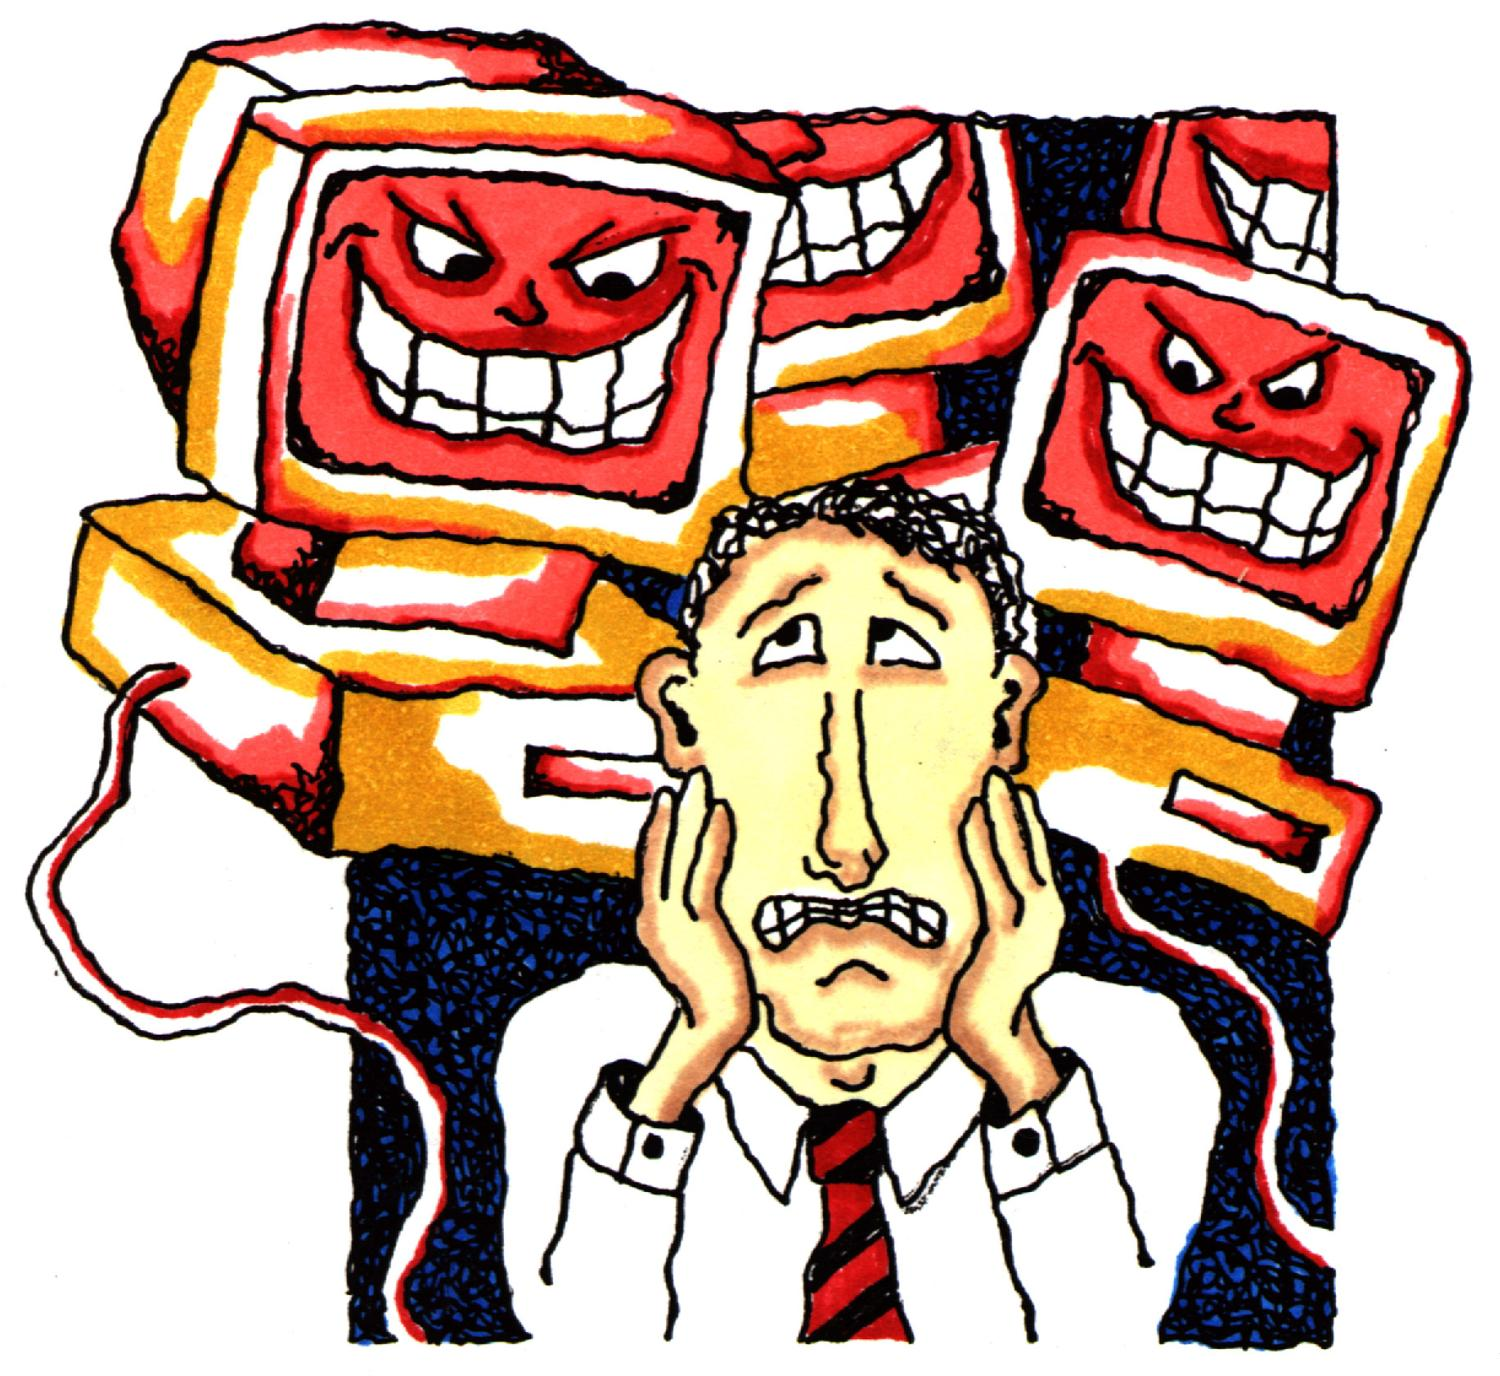
\includegraphics[width=4cm]{../../presentacion/img/malicious}\\
  \end{tabular}
  \end{table}
  \end{frame}
  
  \begin{frame}
  \frametitle{Trust in P2P networks}
  \framesubtitle{Bizantine nodes}
  \begin{table}
  \begin{tabular}{p{7cm}p{3cm}}
  Are all nodes that not behave as expected
  %Multiples causes: connection problems, viruses, modified software, etc.\\
  %\b{\*Nobody can be trusted}
  \begin{enumerate}
      \item Faulty nodes
      \item Malicious nodes
      \item Infected nodes
  \end{enumerate}
  &
  \vspace{1.5cm}
  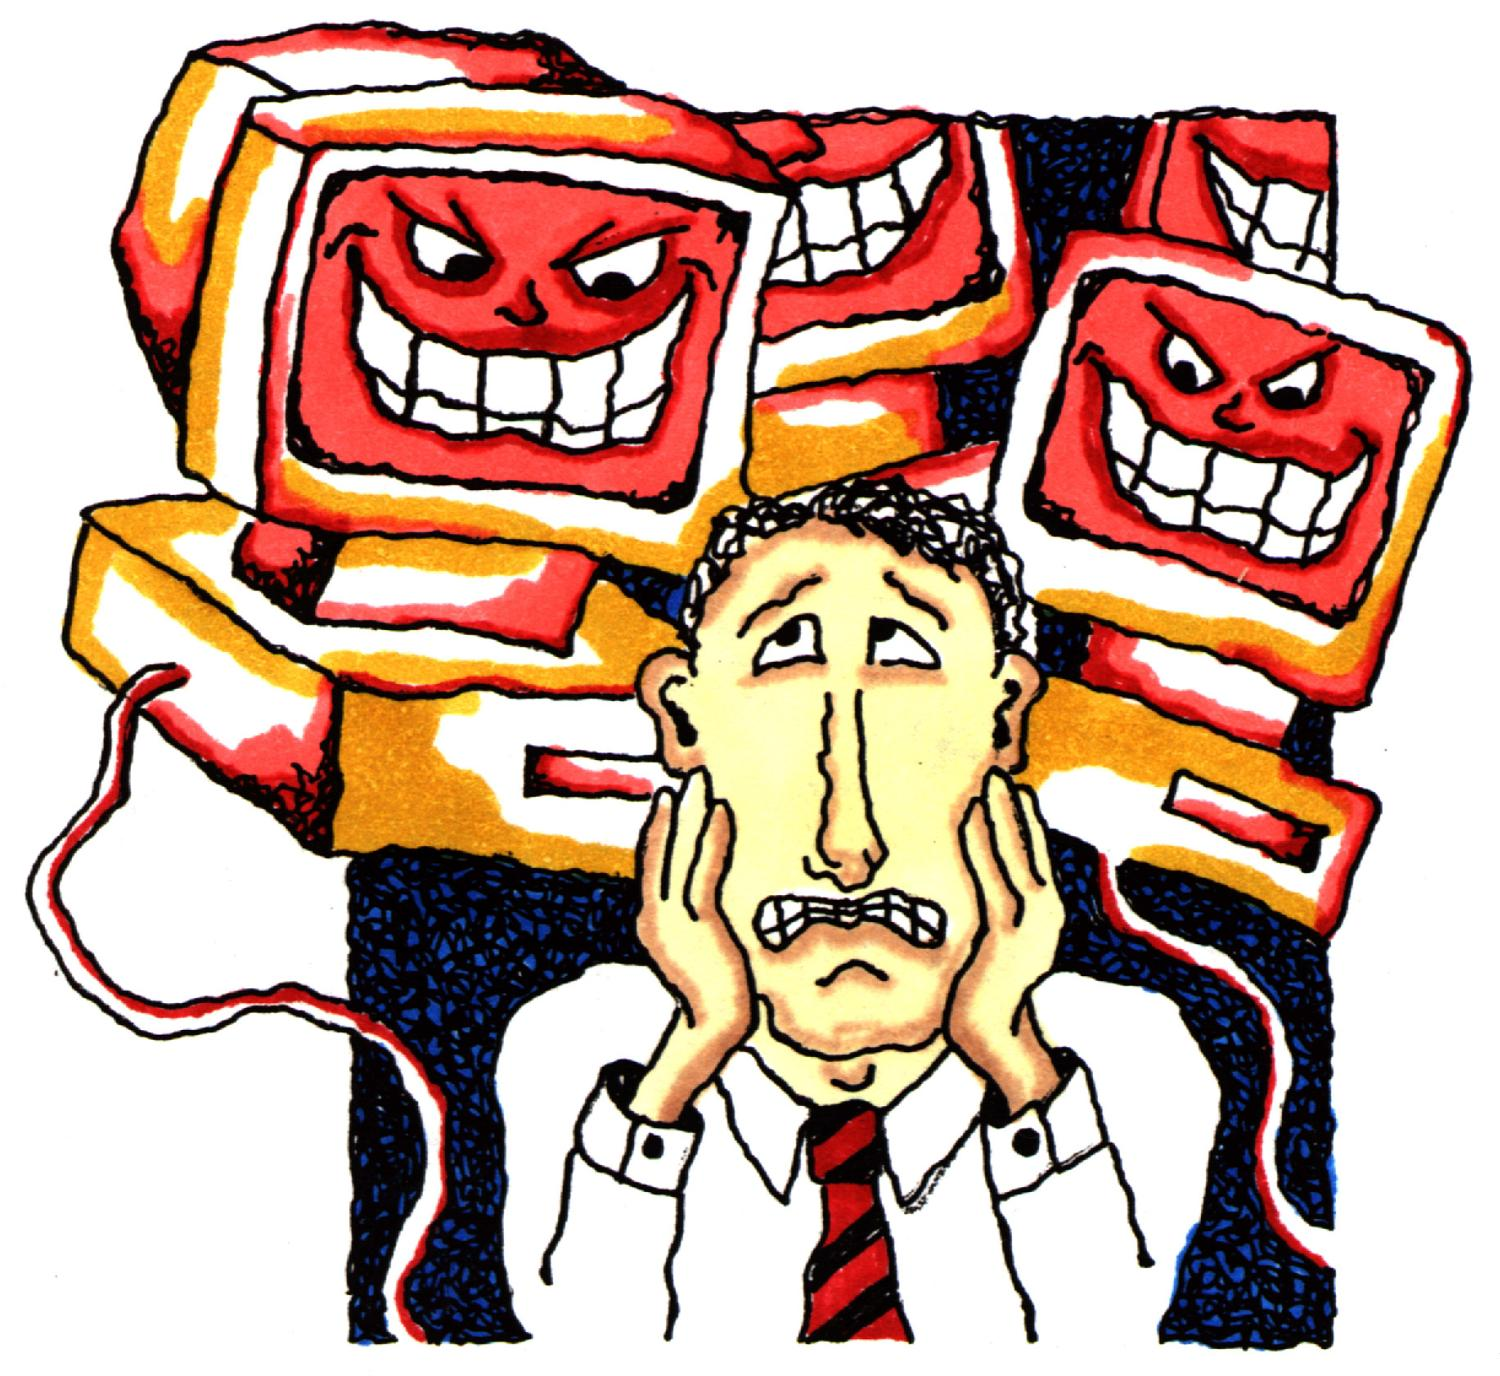
\includegraphics[width=4cm]{../../presentacion/img/malicious}\\
  \end{tabular}
  \end{table}
  \end{frame}
  
  \begin{frame}
  \frametitle{Trust in P2P networks}
  \framesubtitle{Bizantine node tolerance}
  \begin{table}
  \begin{tabular}{p{7cm}p{3cm}}
    P2P networks can achieve byzantine fault tolerance under $1/3$ byzantine
    peers\\
    A peer is honest only if the peers executes the protocol faithfully;
    otherwise, the peer is faulty.
  &
  \vspace{1.5cm}
  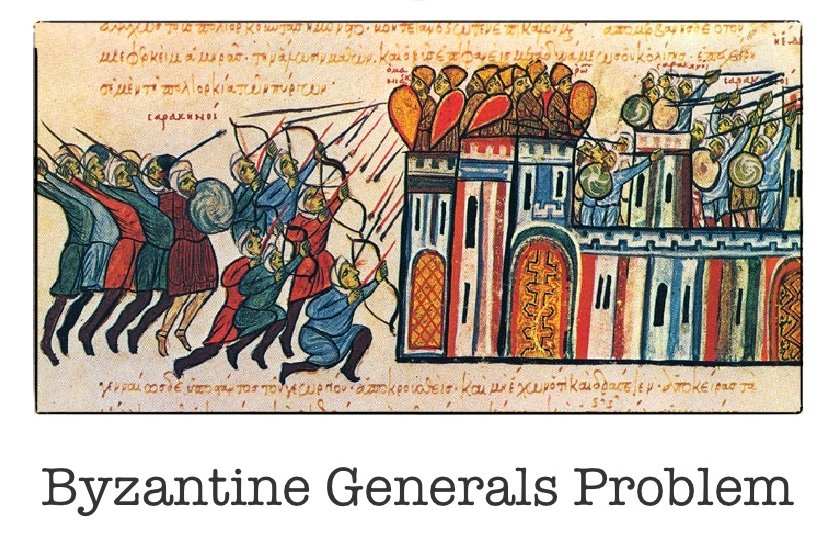
\includegraphics[width=4cm]{../../presentacion/img/bizantine_generals_problem}\\
  \end{tabular}
  \end{table}
  \end{frame}
  
  
  \begin{frame}
  \frametitle{Trust in P2P networks}
  \framesubtitle{Bizantine node tolerance}
  \begin{table}
  \begin{tabular}{p{7cm}p{3cm}}
    P2P networks can achieve byzantine fault tolerance under $1/3$ byzantine
    peers\\
    A peer is honest only if the peers executes the protocol faithfully;
    otherwise, the peer is faulty.
  &
  \vspace{1.5cm}
  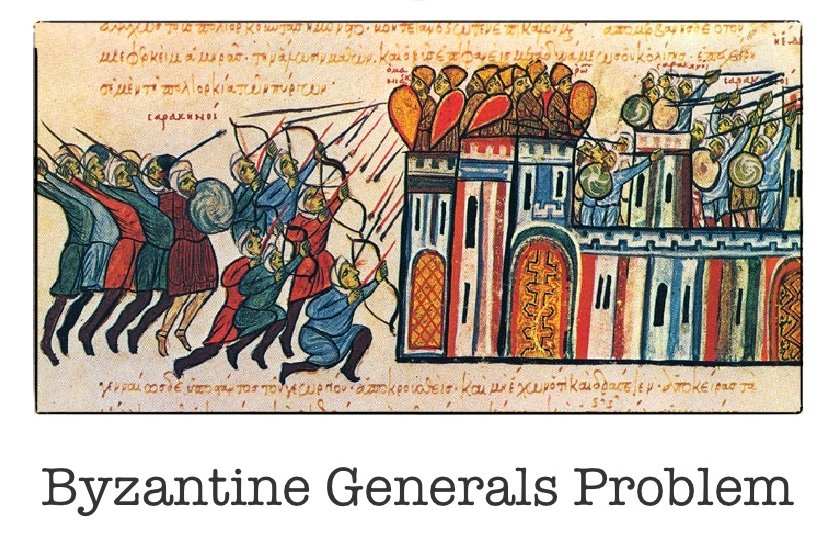
\includegraphics[width=4cm]{../../presentacion/img/bizantine_generals_problem}\\
  \end{tabular}
  \end{table}
  \end{frame}

  %intro of p2p networks


  % identities in P2P networks
  
    % examples

  \subsection{Problem statement}
  % problem for other solutions- multiple devices per user


  \subsection{Thesis proposal}
  %
  %%Before developing an P2P system with the desired functionalities, an adequate
  %%system architecture is needed. We will thoroughly evaluate a new user
  %%identification system that can work in the presence of bizantine nodes, with
  %%the hopes to reach the desirable functionalities with a minimum probability of
  %%failure, to ensure the security of the system in real life scenarios.

  \subsubsection{System architecture}
  % structured p2p and dht based
  % trust management
  % trust-secured protocols
  % criptography schemes

  \section{Working Hypothesis}
    \begin{frame}
    \frametitle{Working Hypothesis}
    %\framesubtitle{Main Goals}
    \begin{table}
    \begin{tabular}{p{7cm}p{3cm}}
      \begin{itemize}
          \item It is assumed that the use of a reputation system and trusted nodes
            management mitigates the efectivity of malicious nodes on identity
            usurpation attacks.
          \item It is assumed that encryption schemes available today are
            sufficient to secure the user's private data in the P2P networks.
      \end{itemize}
    &
    \vspace{1.5cm}
    %\includegraphics[width=4cm]{img/p2p-unstructured}\\
    \end{tabular}
    \end{table}
    \end{frame}

  \section{Goals}
  \subsection{Main Goals}
    \begin{frame}
    \frametitle{Goals}
    \framesubtitle{Main Goals}
    \begin{table}
    \begin{tabular}{p{7cm}p{3cm}}
    The implementation of a secure \textit{username/password} based user identification scheme in structured P2P
    networks using:
    \begin{itemize}
      \item  Secure routing
      \item  Node trust management 
      \item  Encryption schemes
    \end{itemize}
    %\begin{enumerate}
    %    \item Have a minimal possibility of error in the identification process.
    %    \item Use a layer developed scheme that can easily adapt to most commonly
    %          used P2P networks.
    %\end{enumerate}
    &
    \vspace{1.5cm}
    %\includegraphics[width=4cm]{img/p2p-unstructured}\\
    \end{tabular}
    \end{table}
    \end{frame}

  \subsection{Specifics Goals}
    \begin{frame}
    \frametitle{Goals}
    \framesubtitle{Specifics Goals}
    \begin{table}
    \begin{tabular}{p{7cm}p{3cm}}
    \begin{itemize}
      \item Study the possibility of password recovery mechanisms.
      \item Study and use trust management to maintain a
            secure layer inside the P2P network.
      \item Use bizantine tolerant algorithms to verify and maintain the
            system consistency in the presence of malicious nodes.
      \item Study and use secure routing, search and storage mechanisms in
            structured P2P networks.
    \end{itemize}
    &
    \vspace{1.5cm}
    %\includegraphics[width=4cm]{img/p2p-unstructured}\\
    \end{tabular}
    \end{table}
    \end{frame}
  \section{Results}
  \subsection{Contributions and Expected Results}
    \begin{frame}
    \frametitle{Results}
    \framesubtitle{Contributions and Expected Results}
    \begin{table}
    \begin{tabular}{p{7cm}p{3cm}}
      \begin{itemize}
          \item Design of a secure and modern user identification system for
                structured P2P networks.
          \item Generate a base system to develop complex projects in P2P networks.
          \item Reassure that P2P distributed systems have the capabilities to offer
                complex and high level services.
          \item Paper publication.
                %to be sent to a distributed systems
                %publisher. The paper will show the results of the user identification system
                %designed in this project.
      \end{itemize}
    &
    \vspace{1.5cm}
    %\includegraphics[width=4cm]{img/p2p-unstructured}\\
    \end{tabular}
    \end{table}
    \end{frame}

  \subsection{Validation procedures}
    \begin{frame}
    \frametitle{Results}
    \framesubtitle{Validation procedures}
    \begin{table}
    \begin{tabular}{p{7cm}p{3cm}}
      %P2P networks presents a big difficulty to be tested in a real environment
      %because of the high number of nodes needed to try it out.
      %Therefore, instead of going after an empiric validation of the proposed
      %identification system, only a  theoretical evaluation will be presented.
      %The proposed system will be compared with the other systems available at
      %the moment with a thoroughly analysis of the security of the algorithm used.
      %
      %Taking that in consideration, the theoretical evaluation will be focused in:
      %
      \begin{itemize}
          \item Proving that the system will have a minimal probability of error.
          \item Proving that the system will  maintain his consistency in networks with at most 30\% of bizantine nodes. 
      \end{itemize}
    &
    \vspace{1.5cm}
    %\includegraphics[width=4cm]{img/p2p-unstructured}\\
    \end{tabular}
    \end{table}
    \end{frame}

  \section{Bibliography}
  \bibliography{../../../bib/article,../../../bib/paper,../../../bib/url}    %
\frame
{
	\vspace{2cm}
	\begin{center}
		\Large{EOF}
	\end{center}
}
\end{document}
